Neste trabalho, a metodologia será seccionada nas seguintes partes:
\begin{itemize}
    \item  Datasets
    \item  Premissas do problema
    \item  Proposta de solução
    \item  Experimento para a solução do problema

\end{itemize}

Neste capitulo será apresentado em detalhes as premissas do problema de classificação visual bem como a metodologia para sua solução, que será particionada nas conforme proposto a seguir. A seção~\ref{sec:Cap3_Premissas}. apresenta as limitações e condições de contorno do problema. A seção~\ref{sec:Cap3_Dataset} apresenta o conjunto de dados utilizado para o experimento. A seção~\ref{sec:Cap3_Proposta} apresenta a proposta de solução para o problema. A seção~\ref{sec:Cap3_Procedimentos} apresenta os procedimentos do experimento para treino e teste do modelo.

% ----------------------------------------------------------

\section{\textit{Conjunto de dados}}\label{sec:Cap3_Dataset}
Foram utilizados dois pares de conjunto de dados, escolhidos por razões de disponibilidade e representatividade do problema. 

%% Tabelas dos datasets


% ----------------------------------------------------------

\section{\textit{Premissas}}\label{sec:Cap3_Premissas}
Como já mencionado nos capítulo de revisão literária, o problema de localização 
Como premissa, temos dois conjuntos de dados: imagem de satélite ou de voos georreferenciados; e um conjunto de dados correspondente as imagem adquiridas pelo VANT durante o voo. Dessa forma, nossa solução deve receber imagens geolocalizadas para treinar um modelo e retornar as coordenadas de imagens adquiridas durante o voo. 

Vale ressaltar que aqui se encontra a maior dificuldade de generalização, onde as imagens referenciadas e dos drones podem possuir muitas características diferentes: como rotação, escala, altitude, sensor da camera, estação do ano, luminosidade e horário do dia. Além do mais ainda existe a limitação de recursos de hardware dos sistemas embarcados do veículo. E diante disso, a rede deverá ser capaz de estimar a translação do veículo dentro da região de interesse. Outra premissa assumida é a aproximação de região plana, desprezando a curvatura da terra.
% ----------------------------------------------------------

\section{\textit{Proposta de solução}}\label{sec:Cap3_Proposta}

Como solução para o problema, foi proposta a utilização de uma rede neural convolucional que faz a regressão das coordenadas. Se diferencia das soluções de template matching por generalizar a região de interesse, dispensando o armazenamento e comparação de cada medição com todo o mapa, dessa forma reduzindo custo computacional e consumo de recursos do dispositivo. Por esse fato, pode se tornar mais adequada a aplicações embarcadas de drones comerciais com baixas capacidades computacionais. Também para solucionar a questão de limitação de recursos, propõe-se a experimentação de técnicas de compressão e regularização de redes, como pruning e dropout.

TODO: citar o paper de pre-treino
Para solucionar o problema de generalização e dataset limitado da região de interesse, propomos a utilização de um modelo pré-treinado explicado em~\ref{sec:Cap2_transfer} um dataset extensivo de imagens aéreas e de satélites, de forma a aproveitar seu extrator de características, como é realizado em~\cite{Shiguemori2016Embedded}. Assim o modelo será re-treinado para a região de interesse mantendo os pesos das camadas convolucionais congelados e otimizar apenas as ultimas camadas fortemente conectadas, assim como as camadas de saída. 

Dessa forma, a arquitetura proposta é composta por camadas convolucionais e de pooling para undersampling, e que funciona como extrator de características. As camadas seguintes são camadas totalmente conectadas seguidas por uma camada \textit{softmax} que realiza regressão das coordenadas.
% ----------------------------------------------------------

\section{\textit{Ambiente e ferramentas}}\label{sec:Cap3_Ferramentas}


O Ambiente dos experimentos será em cadernos Jupyters, para ser facilmente replicável e ser executável em núvem, com a possiblidade de alugar recursos computacionais no Google Collab. Também será utilizado o framework PyTorch, por razões de disponibilidade de métodos e conhecimentos do autor.

\subsection{\textit{PyTorch}}\label{sec:Cap2_PyTorch}
Pytorch é um framework código aberto de Python para aprendizado de maquinas. É implementado em C++ e CUDA para otimizações de computações numéricas e matriciais, que são extensivas para esta aplicação.
Foi desenvolvido pelo Facebook e é atualmente amplamente adotado pela comunidade de pesquisa e mercado de aprendizado de máquina. Possui muitas implementações das ferramentas mais utilizadas, especificamente aplicadas a \textit{Deep Learning} e visão computacional. Tem ampla adoção devido a intenção de ser um framework de fácil uso e alto nível, com muitas abstrações e técnicas já implementadas.


% ----------------------------------------------------------


% TODO: citar o paper de aplicação direta
\section{\textit{Experimentos}}\label{sec:Cap3_Experimentos}

O trabalho 12 implementa uma CNN com regressão. Enquanto que o trabalho 3 implementa modelos pré-treinados para classificação. Para a construção da nossa solução desejada, tentaremos combinar um modelo pré-treinado com camadas internas e de saída treinadas para a região de interesse.
Consiste em fazer experimentos em uma complexidade crescente, e replicando resultados para garantir corretude. Será simplificado a reprodução para apenas um dataset.
Inicialmente os modelos serão validados com imagens apenas geoespaciais, para em seguida serem validadas nas imagens dos VANTs.

Para obter o modelo proposto e de melhor performance, foi proposto a seguinte sequencia de experimentos para construir o modelo final:
\begin{enumerate}
\item  Replicar experimentos dos trabalhos 2 e 3
\item  Replicar o experimento do trabalho 2 com datasets mencionados em~\ref{sec:Cap3_Dataset}
\item  Replicar o experimento do trabalho 2 com datasets mencionados e modelo pre-treinado
\item Treinar com o mínimo de finetune e validar o experimento anterior com cross validation nos datasets de imagens georeferenciadas (sem os drones)
\item Avaliar performance do anterior com os datasets de imagens de voo de drones
\item Avaliar performance do anterior em um módulo embarcado Nvidia Jetson
\end{enumerate}


    
% ----------------------------------------------------------

\section{\textit{Procedimentos}}\label{sec:Cap3_Procedimentos}

Os procedimentos do experimento principal consiste principalmente nas etapas de 
pré-processamento, treino e validação. Explicadas a diante.

\subsection{\textit{Pré-processamento}}\label{sec:Cap3_PreProcess}
O pré-processamento consistem em preparar as amostras do dataset de interesse para treino e validação. Inicialmente foram geradas 10000 recortes aleatórios de tamanho de imagem aproximadamente ao de angulo de visão do drone na altitude de operação, correspondente a uma área de 100mx100m. Cada recorte é aplicado um \textit{downsampling} para a resolução de entrada do modelo pré-treinado. Para cada recorte é registrado seu respectivo rótulo, que é sua coordenada de latitude e longitude, porem em uma escala de 0 a 1, por meio de um \textit{min-max-scaler}. O \textit{downsampling} offline, durante o treino, é feito por uma interpolação cúbica, enquanto que a online, durante o teste, é feito por uma interpolação bilinear, para alívio de custo computacional, como foi implementado no paper 2.

\subsection{\textit{Treino}}\label{sec:Cap3_Treino}
Para a etapa de treino, utilizamos a arquitetura proposta em~\ref{sec:Cap3_Proposta}, que consiste de um modelo pré-treinado, e substituindo suas ultimas camadas de classificação por camadas fortemente conectadas seguidas de camadas de saída de probabilidade logarítmica, como ilustra a imagem a seguir:


TODO Imagem da arquitetura proposta.

Será treinada utilizando o dataset de imagens geolocalizadas, separados por uma divisão aleatória de 80\% para treino e 20\% para testes, após o pré-processamento. Um valor usual na literatura são 500 épocas, com métrica de distância pela raiz da média do erro quadrático. Será utilizada nas camadas adicionais da rede as técnicas de \textit{dropout e pruning} para realizar regularização e compressão da rede.




\subsection{\textit{Validação}}\label{sec:Cap3_Validacao}

A etapa de validação será realizada a medida do desempenho do modelo no conjunto de testes para regressão.




% Chip (Image) Data Format

% The chips for this competition were derived from Planet's full-frame analytic scene products using our 4-band satellites in sun-synchronous orbit (SSO) and International Space Station (ISS) orbit. The set of chips for this competition use the GeoTiff format and each contain four bands of data: red, green, blue, and near infrared. The specific spectral response of the satellites can be found in the Planet documentation. Each of these channels is in 16-bit digital number format, and meets the specification of the Planet four band analytic ortho scene product.

% For purposes of the competition we have stripped out all of the geotiff information regarding the chip footprint and ground control points (GCPs). The imagery has a ground-sample distance (GSD) of 3.7m and an orthorectified pixel size of 3m. The data comes from Planet's Flock 2 satellites in both sun-synchronous and ISS orbits and was collected between January 1, 2016 and February 1, 2017. All of the scenes come from the Amazon basin which includes Brazil, Peru, Uruguay, Colombia, Venezuela, Guyana, Bolivia, and Ecuador (see map below).

% We have also included a set of JPG chips for reference and practice. These chips were processed using the Planet visual product processor and then saved as jpg chips. These chips are provided as a reference to the scene content, but we expect that the additional information in the tif chips will be more fruitful for the competition.

% https://commons.wikimedia.org/w/index.php?curid=4745680 Above: A map of the Amazon basin.
% Labeling Process and Data Quality

% enter image description here

% To assemble this data set we set out with an initial specification of the phenomena we wished to find and include in the final data set. From that initial specification we created a "wish list" of scenes where we included a ballpark number of scenes required to get a sufficient number of chips to demonstrate the phenomena. This initial set of scenes was painstakingly collected by our Berlin team using Planet Explorer. All told this initial set of scenes numbered approximately 1600 and covered a land area of thirty million hectares.

% This initial set of scenes was then processed using a custom product processor to create the jpg and 4-band tif chips. Any chip that did not have a full and complete four band product was omitted. This initial set of over 150,000 chips was then divided into two sets, a "hard" and an "easy" set. The easy set contained scenes that the Berlin team identified as having easier-to-identify labels like primary rainforest, agriculture, habitation, roads, water, and cloud conditions. The harder set of data was derived from scenes where the Berlin team had selected for shifting cultivation, slash and burn agriculture, blow down, mining, and other phenomenon.

% The chips were labeled using the Crowd Flower platform and a mixture of crowd-sourced labor and our Berlin and San Francisco teams. While the utmost care was taken to get a large and well-labeled dataset, we are aware that not all of the labels in our dataset are correct. Governments around the world retain a large number of highly trained analysts to review images and even they can't always agree on what is present in a given satellite image.

% Moreover, the commonly prescribed approach for labeling data in the GIS community is to use actual ground truth data to label scenes, which is both costly and time consuming. With this in mind we do believe our data has a reasonably high signal to noise ratio and is sufficient for training. Given the ease and expediency of crowd labeling, we believe that a large, relatively inexpensive and rapidly labeled dataset is better than a small, more definitive but less diverse dataset. We are interested to see how competitors handle any inaccuracies.
% Class Labels

% The class labels for this task were chosen in collaboration with Planet's Impact team and represent a reasonable subset of phenomena of interest in the Amazon basin. The labels can broadly be broken into three groups: atmospheric conditions, common land cover/land use phenomena, and rare land cover/land use phenomena. Each chip will have one and potentially more than one atmospheric label and zero or more common and rare labels. Chips that are labeled as cloudy should have no other labels, but there may be labeling errors. Sample chips with labels

% Above: Sample chips and their labels.

% As discussed in the data collection portion of this document, the chip labels are inherently noisy due to the labeling process and ambiguity of features, and scenes may either omit class labels or have incorrect class labels. Part of the challenge of this competition is to figure out how to work with noisy data.
% Cloud Cover Labels

% Clouds are a major challenge for passive satellite imaging, and daily cloud cover and rain showers in the Amazon basin can significantly complicate monitoring in the area. For this reason we have chosen to include a cloud cover label for each chip. These labels closely mirror what one would see in a local weather forecast: clear, partly cloudy, cloudy, and haze. For our purposes haze is defined as any chip where atmospheric clouds are visible but they are not so opaque as to obscure the ground. Clear scenes show no evidence of clouds, and partly cloudy scenes can show opaque cloud cover over any portion of the image. Cloudy images have 90% of the chip obscured by opaque cloud cover.
% Examples of Cloudy Scenes

% Cloudy Scene enter image description here
% Examples of Partly Cloudy Scenes

% Partly Cloudy Scene Partly Cloudy Scene
% Examples of Hazy Scenes

% Partly Cloudy Scene Partly Cloudy Scene
% More Common Labels

% The common labels in this data set are rainforest, agriculture, rivers, towns/cities, and roads. Examples of each class are given below.
% Primary Rain Forest

% The overwhelming majority of the data set is labeled as "primary", which is shorthand for primary rainforest, or what is known colloquially as virgin forest. Generally speaking, the "primary" label was used for any area that exhibited dense tree cover.This Mongobay article gives a concise description of the difference between primary and secondary rainforest, but distinguishing between the two is difficult solely using satellite imagery. This is particularly true in older "secondary" forests. Primary Rainforest

% Above: Approximately 25,000 acres of untouched primary rainforest.
% Water (Rivers & Lakes)

% Rivers, reservoirs, and oxbow lakes are important features of the Amazon basin, and we used the water tag as a catch-all term for these features. Rivers in the Amazon basin often change course and serve as highways deep into the forest. The changing course of these rivers creates new habitat but can also strand endangered Amazon River Dolphins. River

% Above: A larger and slower river with significant sand bars. The brown color comes from significant silt deposits. River

% Above: A small tributary joins a larger river system. The deep brown color of the river is noticeable near the bright sand bars.
% Habitation

% The habitation class label was used for chips that appeared to contain human homes or buildings. This includes anything from dense urban centers to rural villages along the banks of rivers. Small, single-dwelling habitations are often difficult to spot but usually appear as clumps of a few pixels that are bright white. Habitation

% Above: A larger city in the Amazon basin. Habitation

% Above: A large city.
% Agriculture

% Commercial agriculture, while an important industry, is also a major driver of deforestation in the Amazon. For the purposes of this dataset, agriculture is considered to be any land cleared of trees that is being used for agriculture or range land.

% More reading on agriculture in the Amazon:

%     Sugarcane in Bolivia
%     Papaya cultivation destroying Peruvian Rainforest
%     Harvests in Rio Grande do Sul

% Agriculture 1

% Above: An agricultural area that showing the end state of "fishbone" deforestation. Agriculture 2

% Above: A newer agricultural area showing "fishbone" deforestation.
% Road

% Roads are important for transportation in the Amazon but they also serve as drivers of deforestation. In particular, "fishbone" deforestation often follows new road construction, while smaller logging roads drive selective logging operations. For our data, all types of roads are labeled with a single "road" label. Some rivers look very similar to smaller logging roads, and consequently there may be some noise in this label. Analysis of the image using the near infrared band may prove useful in disambiguating the two classes.

% More information: - Roads in the Amazon - NASA article on Fishbone Deforestation

% Road 1

% Above: classic "Fishbone" deforestation following a road. Road 2

% Above: roads snake out of a small town in the Amazon.
% Cultivation

% Shifting cultivation is a subset of agriculture that is very easy to see from space, and occurs in rural areas where individuals and families maintain farm plots for subsistence. This article by MongaBay by MongaBay gives a detailed overview of the practice. This type of agriculture is often found near smaller villages along major rivers, and at the outskirts of agricultural areas. It typically relies on non-mechanized labor, and covers relatively small areas. cultivation

% Above: A zoomed-in area showing cultivation (right side of river) cultivation

% Above: A zoomed-in area showing cultivation and some selective logging. Dark areas indicate recent slash/burn activity
% Bare Ground

% Bare ground is a catch-all term used for naturally occuring tree free areas that aren't the result of human activity. Some of these areas occur naturally in the Amazon, while others may be the result from the source scenes containing small regions of biome much similar to the pantanal or cerrado. bare ground

% Above: a naturally occuring bare area in the cerrado. bare ground

% Above: a naturally occuring bare area in the cerrado.
% Less Common Labels
% Slash and Burn

% Slash-and-burn agriculture can be considered to be a subset of the shifting cultivation label and is used for areas that demonstrate recent burn events. This is to say that the shifting cultivation patches appear to have dark brown or black areas consistent with recent burning.This NASA Earth Observatory article gives a good primer on the practice as does this wikipedia article. Above: ground view of slash and burn agriculture. By Alzenir Ferreira de Souza slash burn

% Above: A zoomed-in view of an area with shifting cultivation with evidence of a recent fire. slash burn

% Above: A zoomed-in view of an area with shifting cultivation and evidence of a recent fire.
% Selective Logging

% The selective logging label is used to cover the practice of selectively removing high value tree species from the rainforest (such as teak and mahogany). From space this appears as winding dirt roads adjacent to bare brown patches in otherwise primary rain forest. This Mongabay Article covers the details of this process. Global Forest Watch is another great resource for learning about deforestation and logging. logging

% Above: The brown lines on the right of this scene are a logging road. Note the small brown dots in the area around the road. logging

% Above: A zoomed image of logging roads and selective logging. logging

% Above: A zoomed image of logging roads and selective logging.
% Blooming

% Blooming is a natural phenomenon found in the Amazon where particular species of flowering trees bloom, fruit, and flower at the same time to maximize the chances of cross pollination. These trees are quite large and these events can be seen from space. Planet recently captured a similar event in Panama. bloom

% Above: a zoomed and contrast enhanced of a bloom event in the Amazon basin. The red arrows point to a few specific trees. The canopies of these trees can be over 30m across (~100ft).
% Conventional Mining

% There are a number of large conventional mines in the Amazon basin and the number is steadily growning. This label is used to classify large-scale legal mining operations.

% mine

% Above: A conventional mine in the Amazon.
% "Artisinal" Mining

% Artisinal mining is a catch-all term for small scale mining operations. Throughout the Amazon, especially at the foothills of the Andes, gold deposits lace the deep, clay soils. Artisanal miners, sometimes working illegally in land designated for conservation, slash through the forest and excavate deep pits near rivers. They pump a mud-water slurry into the river banks, blasting them away so that they can be processed further with mercury - which is used to separate out the gold. The denuded moonscape left behind takes centuries to recover.

%     Illegal and artisanal mines in Peru
%     Images of artisanal mining in Peru
%     MAAP Amazon Report #36
%     MAAP Amazon Report #49
%     Global Forest Watch article on Mining artisanal mine

% Above: A zoomed image of an artisanal mine in Peru. artisanal mine

% Above: A zoomed image of an artisanal mine in Peru.
% Blow Down

% Blow down, also called windthrow, is a naturally occurring phenomenon in the Amazon. Briefly, blow down events occur during microbursts where cold dry air from the Andes settles on top of warm moist air in the rainforest. The colder air punches a hole in the moist warm layer, and sinks down with incredible force and high speed (in excess of 100MPH). These high winds topple the larger rainforest trees, and the resulting open areas are visible from space. The open areas do not stay visible for along as plants in the understory rush in to take advantage of the sunlight.

%     MAAP #55: Blow Down Report in Peru Detailed
%     MAAP #54: Blow Down Report in Peru
%     National Geographic Article on Blow Down
%     Nature article on the size and frequency of blow down events. blow down

% Above: A recent blow down event in the Amazon circled in red. Note the light green of the forest understory and the pattern of tree loss.










% A metodologia para a execução deste trabalho está dividida em três partes, conforme as seções a seguir. A Seção~\ref{sec:Cap3_Deteccao} apresenta a definição do algoritmo selecionado para a resolução do problema de identificação de objetos a partir de imagens, e seu desenvolvimento. Adiante, na Seção~\ref{sec:Cap3_Controle} é explicado como obter parâmetros do manipulador robótico junto ao desenvolvimento de seu controlador. Por fim, a Seção~\ref{sec:Cap3_Simulador} apresenta as estratégias de simulação do sistema a fim de integrar todas as soluções propostas. A Figura~\ref{fig:metodologia} ilustra os principais passos da metodologia.

% \begin{figure}[h!]
%     \centering
%     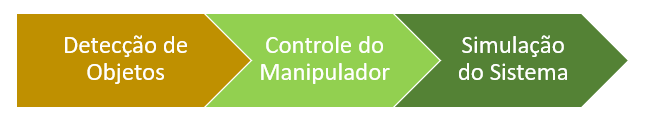
\includegraphics[width=.75\columnwidth]{Imagens/DiagramaMetodologia.PNG}
%     \caption{Metodologia com os principais passos utilizados na execução deste trabalho.}
%     \label{fig:metodologia}
% \end{figure}

% %==============================================================
% \section{\textit{Detecção de Objetos}}\label{sec:Cap3_Deteccao}

% Durante as últimas décadas, foram desenvolvidas muitas tecnologias e \textit{frameworks} voltados para detecção de objetos. Muitos destes são fornecidos de forma paga por empresas do meio, porém existem implementações gratuitas e de qualidade fornecidas por gigantes da indústria tecnológica, e com grande suporte de desenvolvedores independentes. Devido ao suporte e ajuda crescente da comunidade, além da praticidade em suas usabilidades, chegou-se a conclusão que seria mais eficiente a utilização da biblioteca OpenCV~\cite{howse2013opencv}, para a captura das imagens, e TensorFlow~\cite{tensorFlow}, para tratar a identificação de objetos, ambos com suporte para a linguagem de programação Python.

% Em uma primeira etapa, a Subseção~\ref{sec:Cap3_D_OpenCV} irá apresentar um método para captura de imagens que serão tratadas eventualmente. A Subseção~\ref{sec:Cap3_D_TensorFlow} irá contextualizar brevemente a respeito do \textit{framework} TensorFlow e alguns conceitos teóricos de Redes Neurais. Enquanto que a Subseção~\ref{sec:Cap3_D_Modelo} irá apresentar conceitos dos modelos pré-treinados e definir um modelo a ser utilizado a fim de cumprir o propósito deste trabalho.
 
% %-------------------------------------------------------------
% \subsection{\textit{OpenCV}}\label{sec:Cap3_D_OpenCV}
 
% O OpenCV (\textit{Open Source Computer Vision Library}) é uma biblioteca de código aberto que tem foco na visão computacional em tempo real. Ele possui módulos de processamento de imagens e vídeos, e possui uma ampla utilização da comunidade desenvolvedora na utilização de diversas áreas graças a suas ferramentas que permitem filtros, calibração e reconhecimento de padrões. Por mais que ele possa ser utilizado como ferramenta para reconhecimento de objetos em cena, ele foi utilizado neste cenário apenas a captura de imagem em tempo real. Isso se deve a seu processamento ser todo na máquina local, enquanto o TensorFlow possui vantagens que aliviam o custo computacional de todo o processamento.

% A biblioteca foi desenvolvida na linguagem de programação C++, porém existe suporte atualmente para outras linguagens, como Python e Java. O OpenCV está em constante manutenção para agregar melhorias de desempenho e novas funcionalidades, sendo sua última versão estável lançada em abril de 2021. Por se tratar de um código aberto, ele pode ser customizável e explorado a fim de garantir uma funcionalidade ou melhoria que se adeque melhor ao projeto. Para este projeto, entretanto, serão utilizadas funções que já estão integradas à biblioteca.

% Existem atualmente duas versões da biblioteca, sendo a versão 1.0 lançada em 2006 e a versão 2.0 lançada em 2009. A última versão será utilizada neste trabalho, juntamente com suas funções de captura de vídeo a fim de poder armazenar e tratar os quadros de imagens a serem processados.
 
% %-------------------------------------------------------------
% \subsection{\textit{Redes Neurais e TensorFlow}}\label{sec:Cap3_D_TensorFlow}

% Existem muitos elementos da engenharia que foram mimetizados de elementos da natureza e de seres vivos. Um grande exemplo de uma tecnologia nesse sentido que vem sendo amplamente utilizada, são as chamadas Redes Neurais. Elas são modelos computacionais que se inspiram na funcionalidade dos neurônios para realização de Aprendizado de Máquina, tal como Reconhecimento de Padrões.

% Assim como os humanos aprendem a reconhecer coisas na natureza a partir de treinamentos de discernimento, as Redes Neurais passam pelo mesmo processo, realizando uma iteração com ajustes aplicados em seus pesos, a qual é chamada de treinamento. Sua composição é realizada por nós e arestas, que são análogos a neurônios e sinapses, respectivamente.

% Inicialmente, alguns dados são percorridos ao longo do sistema para que possam ser gerados informações comparativas. Após essa etapa, o sistema está pronto para receber novos dados para comparar com os já conhecidos, a fim de gerar um resultado da iteração. Dessa forma, as arquiteturas podem ser classificadas como: Camada de Entrada, Camada Escondida ou Intermediária, e Camada de Saída. A primeira está relacionada com a inserção dos padrões apresentados. O processamento de dados ocorrem majoritariamente na Camada Intermediária, onde existe um maior fluxo de arestas e nós. O resultado é disponibilizado na Camada de Saída. O esquemático representando a estrutura pode ser observado na Figura~\ref{fig:RedeNeural}.

% \begin{figure}[h!]
%     \centering
%     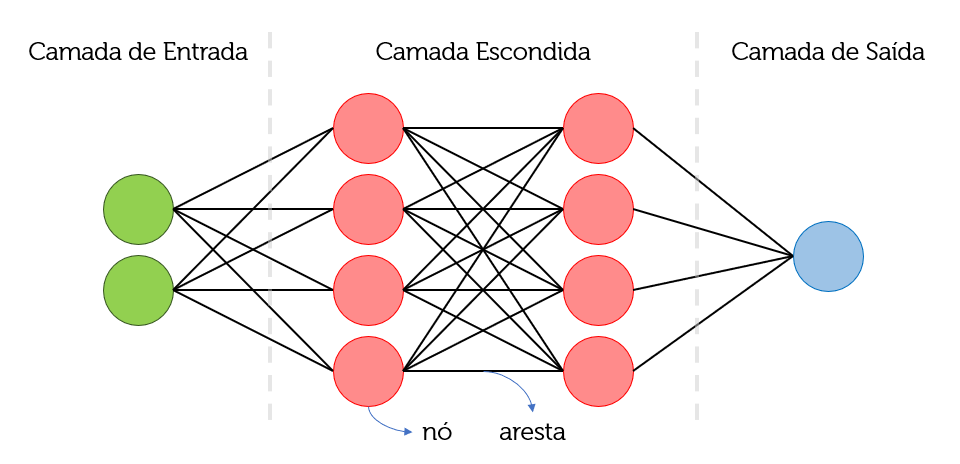
\includegraphics[width=.75\columnwidth]{Imagens/RedeNeural.PNG}
%     \caption{Estrutura organizacional de uma Rede Neural.}
%     \label{fig:RedeNeural}
% \end{figure}

% O TensorFlow é um exemplo de ambiente de código aberto para uso de Aprendizado de Máquina que foi desenvolvido pela Google. Ele vem sido bastante utilizado para soluções tecnológicas de muitas empresas nos últimos tempos, como a Coca-Cola~\cite{brandt_how_2017}, a GE~\cite{polzin_intelligent_2019} e a própria Google~\cite{bendersky_google_2021}. Por ser uma aplicação gratuita e de fácil uso de Redes Neurais, e por apresentar uma comunidade ativa e com suporte por parte dos desenvolvedores, o \textit{framework} se tornou uma alternativa agradável para desenvolver e treinar modelos de aprendizado.

% A maior vantagem do TensorFlow para este projeto é a sua flexibilidade. Ele foi criado para ser executado em diversas plataformas e sistemas operacionais, sejam estes os tradicionais computadores ou dispositivos móveis. De acordo com o modelo a ser treinado, ele pode ser executado por uma CPU\footnote{CPU: \textit{Central Process Unit}}, uma GPU\footnote{GPU: \textit{Graphics Processing Unit}} ou uma TPU\footnote{TPU: \textit{Tensor Processing Unit}}, esta última sendo uma criação da própria Google para ser utilizada junto ao TensorFlow. A biblioteca permite que execute todo o processamento de forma local, em um computador ou dispositivo móvel, além de permitir um processamento na nuvem, o que se faz bem útil para aqueles que não possuem um hardware potente.


% %-------------------------------------------------------------
% \subsection{\textit{Modelo pré-treinado}}\label{sec:Cap3_D_Modelo}

% Através de um banco de dados, é possível treinar um modelo com o TensorFlow. A Google disponibiliza uma página\footnote{TensorFlow: \url{https://www.tensorflow.org/}} com o suporte para todo o processo, porém a biblioteca também permite a utilização de modelos pré-treinados para que sejam utilizados por outros membros da comunidade desenvolvedora.
% % Estes modelos reduzem o tempo desempenhado no projeto e são capazes de apresentar resultados melhores do que se produzidos com outros bancos de dados. Muitos destes modelos são constantemente atualizados para prover melhorias, sendo alguns deles disponibilizados na própria página do TensorFlow.

% Neste trabalho foi utilizado como modelo o COCO-SSD. Trata-se de um modelo pré-treinado desenvolvido e envelopado por desenvolvedores do Google capaz de identificar múltiplos objetos diferentes em uma imagem. O modelo consegue identificar 90 objetos diferentes~\cite{noauthor_pre-trained_2021} que podem ser encontrados no cotidiano. Seu nome vem da junção de duas siglas: COCO e SSD. COCO (\textit{Common Objects in Context}) é um dataset construído pela Microsoft que foi utilizado para treinamento, sendo disponibilizado gratuitamente com mais de 200 mil imagens. Já SSD (\textit{Single Shot Detector}) é um detector de objetos que é capaz de identificar as diferentes classes de objetos.~\cite{forson_understanding_2019}.

% \begin{figure}[b!]
% \centering
% \includegraphics[width=0.7\columnwidth]{Imagens/BoundaryBox.jpeg}
% \caption{Caixa delimitadora mínima na utilização do COCO-SSD.~\cite{mayes_make_2021}}
% \label{fig:cocossd}
% \end{figure}

% O COCO-SSD é capaz de identidicar diferentes objetos em uma mesma imagem, mesmo que sobrepostos. Para isso, ele cria uma caixa delimitadora mínima que é capaz de envolver o objeto com a menor medida de identificação possível. Além disso, ele identifica um nível de confiabilidade do objeto identificado no topo das caixa a partir de uma porcentagem. Um exemplo pode ser observado na Figura~\ref{fig:cocossd}.

% % \begin{figure}[b!]
% % \centering
% % \includegraphics[width=0.7\columnwidth]{src/imgs/BoundaryBox.jpeg}
% % \caption{Caixa delimitadora mínima na utilização do COCO-SSD.}
% % \label{fig:cocossd}
% % \end{figure}

% O algoritmo de detecção de objetos do TensorFlow foi incorporado a um \textit{script} desenvolvido para a solução do problema proposto neste trabalho. O \textit{script} tem como entrada a imagem capturada pela câmera e armazenada através de funções disponíveis pelo OpenCV. Como saída, o \textit{script} retorna os vértices das posiçãos onde foram detectadas as pessoas na imagem. Estes dados serão tratados e servirão de base para o posicionamento desejado do efetuador do manipulador robótico.


% %===========================================================
% \section{\textit{Controle de Manipulador Robótico}}\label{sec:Cap3_Controle}

% Os Manipuladores Robóticos são capazes de administrar tarefas com boa precisão, além de automatizar processos. A componente de maior importância em um manipulador é, em muitas vezes, o efetuador, a qual se encontra em um extremo, e é capaz de se movimentar dentro de uma área de trabalho e exercer funções pré-determinadas. Isso pode ser apresentado na Figura~\ref{fig:workspace}, a qual a região hachurada representa a área de trabalho em que o efetuador pode operar.

% \begin{figure}[h!]
% \centering
% 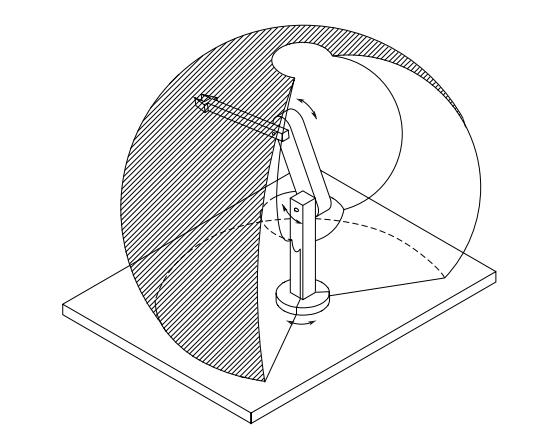
\includegraphics[width=0.7\columnwidth]{Imagens/workspace.PNG}
% \caption{Área de trabalho de um Manipulador Robótico.~\cite{siciliano2010robotics}}
% \label{fig:workspace}
% \end{figure}

% Em uma primeira etapa, a Subseção~\ref{sec:Cap3_Espacial} irá apresentar conceitos importantes que serão utilizados no controle do manipulador. A Subseção~\ref{sec:Cap3_CinDir} irá definir métodos utilizados para leitura de pose do manipulador, enquanto a subseção~\ref{sec:Cap3_CinDif} irá definir métodos para leitura de velocidade. Por fim, a Subseção~\ref{sec:Cap3_ControleCin} irá apresentar técnicas de controle que irão utilizar de dados que foram apresentados na Seção~\ref{sec:Cap3_Deteccao}.

% %-------------------------------------------------------------
% \subsection{\textit{Descrição Espacial}}\label{sec:Cap3_Espacial}

% Para compreender o comportamento dos elementos de um manipulador robótico, é necessário saber como eles são descritos dentro de um espaço tridimensional a qual será servirá para localização no espaço real dos objetos. Primeiro, é preciso definir um ponto de origem que seja comum a todos os objetos que serão representados no cenário. Além disso, é necessário definir os eixos $x$, $y$ e $z$, que são ortogonais entre si, e que possuem origem no ponto citado. Esses dados serão úteis para definição de posição e orientação do objeto no cenário.

% \begin{figure}[h!]
% \centering
% 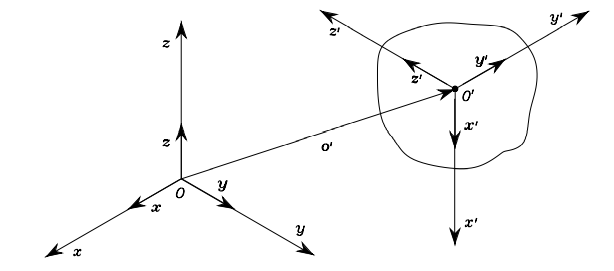
\includegraphics[width=0.7\columnwidth]{Imagens/PosEOri.PNG}
% \caption{Posição e orientação de um objeto no cenário.~\cite{siciliano2010robotics}}
% \label{fig:PoseOri}
% \end{figure}

% Pode-se perceber pela Figura~\ref{fig:PoseOri} que a posição de um objeto na posição do ponto $O'$ pode ser expressa com relação ao ponto e coordenadas de origem como:

% \begin{equation}
% o' = o'_xx+o'_yy+o'_zz
% \label{eq:3_01}
% \end{equation}

% Uma vez que $o'_x$, $o'_y$ e $o'_z$ são componentes do vetor $o'\in \mathbf{R}^3$, a posição de $O'$ pode ser descrita de acordo com o seguinte vetor (3x1):

% \begin{equation}
% o' = 
% \begin{bmatrix}
% o'_x & o'_y & o'_z
% \end{bmatrix} ^T
% \label{eq:3_02}
% \end{equation}

% Para descrever a orientação do objeto, é adequado considerar eixos ortogonais que serão deslocados em referência aos eixos da origem. Dessa forma, os eixos podem ser representados pelas seguintes expressões:

% \begin{equation}
% \begin{matrix}
% x' = x'_xx+x'_yy+x'_zz\\
% y' = y'_xx+y'_yy+y'_zz\\
% z' = z'_xx+z'_yy+z'_zz
% \end{matrix}
% \label{eq:3_03}
% \end{equation}

% Descrevendo a Equação~\ref{eq:3_03} como um vetor (3x3), é possível obter a matriz de rotação ($Q$) do objeto, que é definida pela Equação~\ref{eq:3_04}.

% \begin{equation}
% Q = 
% \begin{bmatrix}
% x' & y' & z'
% \end{bmatrix}  = 
% \begin{bmatrix}
% x'_x & y'_x & z'_x \\
% x'_y & y'_y & z'_y \\
% x'_z & y'_z & z'_z
% \end{bmatrix}  = 
% \begin{bmatrix}
% x'^Tx & y'^Tx & z'^Tx \\
% x'^Ty & y'^Ty & z'^Ty \\
% x'^Tz & y'^Tz & z'^Tz
% \end{bmatrix}
% \label{eq:3_04}
% \end{equation}

% É importante pontuar que, aplicando uma orientação que segue os fundamentos da regra da mão direita, o determinante da matriz será de tal forma que $det(Q) = 1$. A estrutura que compõe a posição e rotação de um objeto dado um determinado tempo, é chamada de referencial – também conhecido como \textit{frame}.

% % \begin{figure}[h!]
% % \centering
% % \includegraphics[width=0.7\columnwidth]{Imagens/DoisPontos.PNG}
% % \caption{Vetores de posição dado dois objetos e \textit{referência mundo}.}
% % \label{fig:DoisPontos}
% % \end{figure}

% Quando existe mais de um objeto em um dado cenário, é possível representar os objetos com relação a origem ou com relação entre si. Para isso, define-se o vetor de posição dos vértices como $p_O^D$, sendo $O$ o ponto de origem e $D$ o ponto de destino do vetor. Isso pode ser melhor avaliado na Figura~\ref{fig:DoisPontos}. Há técnicas dentro da robótica que utilizam os vetores sempre com relação ao chamado \textit{referência mundo}, que serve de referência universal para todos os objetos do cenário; enquanto outros adotam referências sempre de acordo com o objeto anterior analisado.

% \begin{figure}[h!]
% \centering
% \includegraphics[width=0.7\columnwidth]{Imagens/DoisPontos.PNG}
% \caption{Vetores de posição dado dois objetos e \textit{referência mundo}.}
% \label{fig:DoisPontos}
% \end{figure}

% % \begin{figure}[b!]
% % \centering
% % \includegraphics[width=0.7\columnwidth]{src/imgs/DoisPontos.PNG}
% % \caption{Vetores de posição dado dois objetos e \textit{referência mundo}.~\cite{siciliano2010robotics}}
% % \label{fig:DoisPontos}
% % \end{figure}

% Uma notação muito comum no campo da robótica é a Matriz de Transformação Homogênea. Com ela, é possível demonstrar a posição e orientação de um objeto dado uma referência. Ela é composta pela matriz de rotação ($Q$), vetor de posição ($p$) e preenchida por valores nulos e unitários para que a matriz possa ser quadrada. Dessa forma, a Matriz de Transformação Homogênea ($H_{4x4}$) pode ser representada pela Equação~\ref{eq:3_05}.

% \begin{equation}
% H_0^1 = 
% \begin{bmatrix}
% Q_0^1 & p_0^1 \\
% 0_{1x3} & 1
% \end{bmatrix} 
% \label{eq:3_05}
% \end{equation}

% O objeto pode sofrer transformações de rotação e posição, e é necessário definir a leitura da ordem das ações tomadas. Dado um produto $T = R_x(\pi)R_z(\pi/2)$, pode-se ler a transformação da direita para a esquerda, ou da esquerda para a direita. No primeiro cenário, irá ocorrer uma rotação de $\pi/2$ no eizo $z_0$ e depois uma rotação de $\pi$ em $x_0$. No segundo cenário, irá ocorrer uma rotação de $\pi$ no eizo $x_0$ e depois uma rotação de $\pi/2$ em $z_1$. Perccebe-se então que a ordem influencia no estado do \textit{frame} final, sendo o primeiro cenário considerando o \textit{frame 0} como referência, e no segundo, considerando o \textit{frame} anterior.

% Com os conceitos de descrição espacial definidos, é possível conhecer mais sobre a Cinemática Direta a fim de obter os dados dos \textit{frames} de um manipulador robótico.

% %-------------------------------------------------------------
% \subsection{\textit{Cinemática Direta}}\label{sec:Cap3_CinDir}

% A Cinemática permite estudar os movimentos dos manipuladores sem a necessidade de tratar força e torque em suas análises. Para este estudo, se usa o conceito de Espaço de Configurações, normalmente denotado por $Q$. Ele é o conjunto de todas as configurações de um sistema, sendo cada configuração um conjunto de coordenadas que permite identificar uma partícula do manipulador no espaço. A configuração é denotada por $q$, e pode ser representada por coordenadas cartesianas, polares, entre outras.

% Definindo um \textit{frame} de \textit{referência mundo}, pode-se descrever o estado atual do \textit{frame} do efetuador a partir do deslocamento de juntas prismáticas e/ou rotação de juntas rotativas. É possível definir uma função de Cinemática Direta do frame desejado, sendo esta uma função da configuração $q$, como pode ser observado na Equação~\ref{eq:3_06}.

% \begin{equation}
% T = f(q)
% \label{eq:3_06}
% \end{equation}

% A Convenção de Denavit-Hartenberg é muito utilizada na área da robótica para definir a Cinemática Direta de um manipulador. Ela define regras para criação de referenciais intermediários ao longo do manipulador de forma que facilite a transformação de um referencial de origem – geralmente utilizando o \textit{referencial do mundo} – para um referencial final desejado.

% Para isso, é necessário definir alguns conceitos:

% \begin{itemize}
% \item $elo_i:$ \textit{i}-ésimo elo.
% \item $reta_i:$ reta alinhada com o eixo de rotação/translação \textit{i}, afixada ao $elo_i$. 
% \item $pontoA_i:$ ponto da $reta_i$ mais próximo de $reta_{i+1}$.
% \item $pontoB_i:$ ponto da $reta_{i+1}$ mais próximo de $reta_i$.
% \item $frame_i:$ eixo afixado no $elo_i$.
% \end{itemize}

% Definido os conceitos, é aplicado um método geral para a convenção, sendo $i$ o número da junta analisada no atual momento. Dessa forma, aplica-se a seguinte ordem de ações:

% \begin{enumerate}
% \item Traçar a $reta_i$ e a $reta_{i+1}$.
% \item Encontrar o $pontoA_i$ e o $pontoB_i$.
% \item O $frame_{i+1}$ estará centrado no $pontoB_i$.
% \item É convencionado que o eixo $z_i$ está alinhado com o eixo de rotação/deslocamento da $reta_i$.
% \item Alinha-se o eixo $z_i$ com relação ao próximo eixo de rotação/deslocamento, da $reta_{i+1}$.
% \item O eixo $x_i$ tem seu sentido inicial arbitrário.
% \item Alinha-se o eixo $x_i$ no sentido de $pontoA_i$ para $pontoB_i$.
% \item Aplicando a regra da mão direita, define-se o eixo $y_i$.
% \end{enumerate}

% Por fim, define-se as variáveis de rotação e trasnalação, sendo estas:

% \begin{itemize}
% \item $a_i:$ translação no eixo $x$.
% \item $\alpha_i:$ rotação no eixo $x$. 
% \item $d_i:$ translação no eixo $z$.
% \item $\vartheta_i:$ rotação no eixo $z$. 
% \end{itemize}

% Aplicando as regras acima no braço antropomórfico da Figura~\ref{fig:BracoAntro} como exemplo, é possível obter os parâmetros de Denavit-Hartenberg descritos na Tabela~\ref{table:3_01}.

% \begin{figure}[b!]
% \centering
% 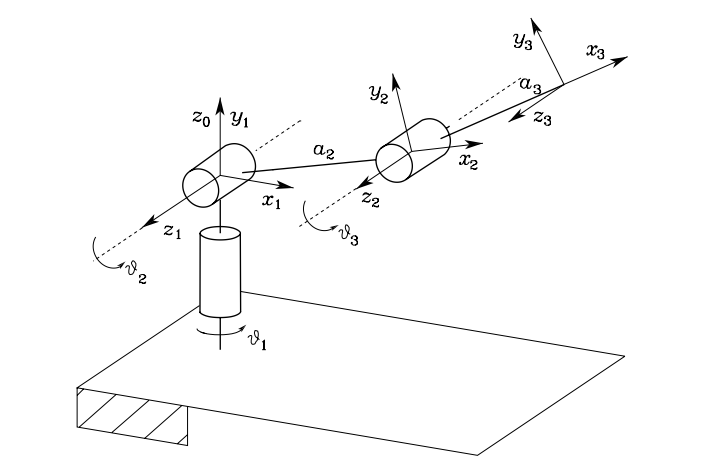
\includegraphics[width=0.7\columnwidth]{Imagens/BracoAntropo.PNG}
% \caption{Braço antropomórfico.\cite{siciliano2010robotics}}
% \label{fig:BracoAntro}
% \end{figure}

% \begin{table}[h!]
% \centering
% \begin{tabular}{c|c|c|c|c}
%  \hline
%  Elo & $a_i$ & $\alpha_i$ & $d_i$ & $\vartheta_i$ \\ [0.5ex] 
%  \hline\hline
%  1 & 0 & $\pi$/2 & 0 & $\vartheta_1$ \\ 
% %  \hline
%  2 & $a_2$ & 0 & 0 & $\vartheta_2$ \\ 
% %  \hline
%  3 & $a_3$ & 0 & 0 & $\vartheta_3$ \\ 
%  \hline
% \end{tabular}
% \caption{Parâmetros de Denavit-Hartenberg para o braço antropomórfico.}
% \label{table:3_01}
% \end{table}

% Considerando $cos(\vartheta_i)$ como $c_i$ e $sen(\vartheta_i)$ como $s_i$, é possível definir as Matrizes de Transformação Homogêneas da seguinte forma:

% \begin{equation}
% H_0^1 (\vartheta_1) = 
% \begin{bmatrix}
% c_1 & 0 & s_1 & 0 \\
% s_1 & 0 & -c_1 & 0 \\
% 0 & 1 & 0 & 0 \\
% 0 & 0 & 0 & 1 \\
% \end{bmatrix} 
% \label{eq:3_07}
% \end{equation}

% \begin{equation}
% \begin{matrix}
% H_{i-1}^i (\vartheta_i) = 
% \begin{bmatrix}
% c_i & -s_i & 0 & 0 \\
% s_i & c_i & 0 & 0 \\
% 0 & 0 & 1 & 0 \\
% 0 & 0 & 0 & 1 \\
% \end{bmatrix} & i = 2,3
% \end{matrix}
% \label{eq:3_08}
% \end{equation}

% Assim, a função de Cinemática Direta descrita na Equação~\ref{eq:3_06}, onde $q = \begin{bmatrix}\vartheta_1 & \vartheta_2 & \vartheta_3\end{bmatrix}^T$, pode ser representada por:

% \begin{equation}
% T_0^3 (q) = 
% H_0^1 H_1^2 H_2^3 = 
% \begin{bmatrix}
% c_1 c_{23} & -c_1 s_{23} & s_1 & c_1(a_2 c_2 + a_3 c_{23}) \\
% s_1 c_{23} & -s_1 s_{23} & c_1 & s_1(a_2 c_2 + a_3 c_{23}) \\
% s_{23} & c_{23} & 0 & a_2 s_2 + a_3 s_{23} \\
% 0 & 0 & 0 & 1 \\
% \end{bmatrix} 
% \label{eq:3_09}
% \end{equation}

% %-------------------------------------------------------------
% \subsection{\textit{Cinemática Diferencial}}\label{sec:Cap3_CinDif}

% A Cinemática Direta permite obter o valor de pose de um \textit{frame} desejado dado a configuração $q$ de um manipulador. Adicionando a informação da velocidade da configuração, é possível determinar a velocidade do \textit{frame} do efetuador através da Cinemática Diferencial. Para isso, é importante se ater a propriedades importantes de matrizes e como manipulá-las.

% Uma matriz quadrada que é oposta de sua transposta, ou seja, $S^T = -S$, é chamada de matriz antissimétrica. Dado um vetor $\omega(t) = \begin{bmatrix}\omega_x & \omega_y & \omega_z\end{bmatrix}^T \in \mathbf{R}^3$, pode-se definir uma matriz antissimétrica $S(t)$, como descrito na Equação~\ref{eq:3_10}, sendo $S(t) = S(\omega(t))$.

% \begin{equation}
% S = 
% \begin{bmatrix}
% 0 & -\omega_z & \omega_y\\
% \omega_z & 0 & -\omega_x \\
% -\omega_y & \omega_x & 0 \\
% \end{bmatrix} 
% \label{eq:3_10}
% \end{equation}

% Sabe-se que um produto matricial utilizando uma matriz antissimétrica $S_{3x3}$ pode ser representado por um produto vetorial utilizando elementos da matriz. Assim, considerando $p$ como um vetor tridimensional coluna, é possível afirmar a propriedade descrita na Equação~\ref{eq:3_11}.

% \begin{equation}
% S(\omega)p = \omega \times p
% \label{eq:3_11}
% \end{equation}

% É importante ressaltar que a anticomutatividade do produto vetorial ainda está presente nas propriedades aplicadas a matrizes antissimétricas. Isso pode ser observado através das relações da Equação~\ref{eq:3_12}.

% \begin{equation}
% S(\omega)p = \omega \times p = -(p \times \omega) = -S(p)\omega
% \label{eq:3_12}
% \end{equation}

% Ainda, considerando uma matriz de rotação $Q(t)$, é possível definir um vetor $\omega(t)\in \mathbf{R}^3$ de forma que a Equação~\ref{eq:3_13} seja coerente.

% \begin{equation}
% \frac{dQ(t)}{dt} = S(\omega(t)) Q(t)
% \label{eq:3_13}
% \end{equation}

% O efetuador pode assumir dois tipos de velocidades: velocidade linear, $\dot{p}_e$; e velocidade angule, $\omega_e$. Ambas são funções das velocidades das juntas, $\dot{q}$. Através de matrizes jacobianas, pode-se traçar uma relação linear entre a velocidades das juntas e a velocidade linear e angular do efetuador, sendo esta relação demonstrada na Equação~\ref{eq:3_14}.

% \begin{equation}
% v_e = 
% \begin{bmatrix}
% \dot{p}_e\\
% \omega_e\\
% \end{bmatrix} = J_{geo}(q)\dot{q}
% \label{eq:3_14}
% \end{equation}

% Sendo $J_{geo}(q)$ composto pela Jabiana de posição $J_p(q)$, uma matrix $(3 \times n)$ que relaciona com a velocidade linear $\dot{p}_e$, e pela Jabiana de orientação $J_{\omega}(q)$, uma matrix $(3 \times n)$ que relaciona com a velocidade angular $\omega_e$, sendo $n$ o número de juntas do manipulador. Isso pode ser melhor representado pela Equação~\ref{eq:3_15}.

% \begin{equation}
% J_{geo} = 
% \begin{bmatrix}
% J_p\\
% J_{\omega}\\
% \end{bmatrix}
% \label{eq:3_15}
% \end{equation}

% Se tratando de um corpo rígido, como o elo que conecta a junta ao efetuador, há algumas análises que podem ser feitas a fim de compreender melhor a influência das velocidades. Dado a Figura~\ref{fig:CorpoRig}, é possível notar que o objeto possui um frame em seu centro, representado pelo ponto $p_c$, e uma partícula $P$ afixada em seu corpo rígido. A posição da partícula ao longo do tempo pode ser representada pela Equação~\ref{eq:3_16}, a qual possui informações da posição do centro do objeto e a posição da partícula com relação ao centro dada uma matriz de rotação.

% \begin{equation}
% p^P_0 = Q(t)p^P_{obj} + p_c(t)
% \label{eq:3_16}
% \end{equation}

% \begin{figure}[t!]
% \centering
% 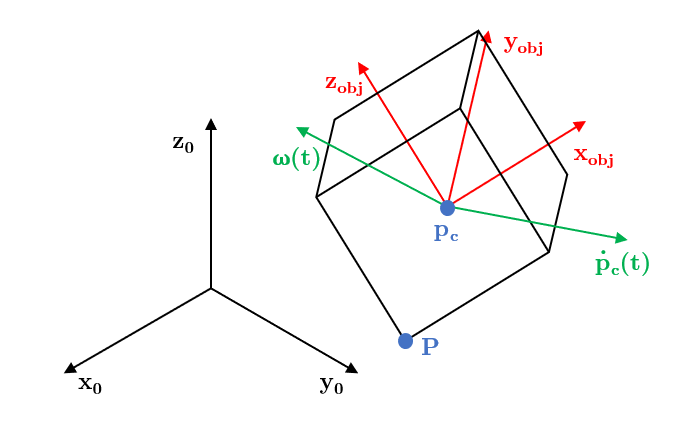
\includegraphics[width=0.7\columnwidth]{Imagens/CorpoRig.PNG}
% \caption{Corpo rígido com vetores de velocidade linear e angular.}
% \label{fig:CorpoRig}
% \end{figure}

% Derivando a Equação~\ref{eq:3_16} ao longo do tempo, pode-se obter a relação dada pela Equação~\ref{eq:3_17}. Utilizando da propriedade apresentada na Equação~\ref{eq:3_13}, e realizando uma relação vetorial das posições dos pontos de origem, central e da partícula, é possível obter as igualdades dadas pela Equação~\ref{eq:3_18} e~\ref{eq:3_19}.

% \begin{equation}
% \dot{p}^P_0 = \dot{Q}(t)p^P_{obj} + \dot{p}_c(t)
% \label{eq:3_17}
% \end{equation}

% \begin{equation}
% \dot{p}^P_0 = S(\omega(t))Q(t)p^P_{obj} + \dot{p}_c(t)
% \label{eq:3_18}
% \end{equation}

% \begin{equation}
% \dot{p}^P_0 = S(\omega(t))(p^P_0(t) - p_c(t)) + \dot{p}_c(t)
% \label{eq:3_19}
% \end{equation}

% Por fim, aplicando a propriedade apresentada na Equação~\ref{eq:3_18} e aplicando na Equação~\ref{eq:3_19}, é possível obter um produto vetorial que pode ser observado pela Equação~\ref{eq:3_20}.

% \begin{equation}
% \dot{p}^P_0 = \omega(t) \times (p^P_0(t) - p_c(t)) + \dot{p}_c(t)
% \label{eq:3_20}
% \end{equation}

% Assim, pode-se observar a contribuição da velocidade angular da partícula através de $\omega(t) \times (p^P_0(t) - p_c(t))$, enquanto a contribuição da velocidade linear se dá por $\dot{p}_c(t)$. Dessa forma, é possível traçar as jacobianas de posição e orientação a fim de analisar ambas as velocidades em uma relação linear com as velocidades das configurações. Omitindo a variável $t$ para tornar o processo mais simples de compreensão, e considerando $R_x(q)$, $R_y(q)$ e $R_z(q)$ as linhas da matriz $Q$, as jacobianas podem ser representadas pelas Equações~\ref{eq:3_21} e~\ref{eq:3_22}.

% \begin{equation}
% J_p(q) = \frac{\partial p_c}{\partial q}
% \label{eq:3_21}
% \end{equation}

% \begin{equation}
% J_{\omega}(q) =
% \begin{bmatrix}
% R_y(q)^T \frac{\partial R_z(q)}{\partial q}\\
% R_z(q)^T \frac{\partial R_x(q)}{\partial q}\\
% R_x(q)^T \frac{\partial R_y(q)}{\partial q}\\
% \end{bmatrix}
% \label{eq:3_22}
% \end{equation}

% Analisando do ponto de vista do efetuador, e utilizando as relações apresentadas acima, é possível determinar as matrizes jacobianas do efetuador. Seja $n$ o \textit{frame} da última junta antes do efetuador, é possível definir as relações das Equações~\ref{eq:3_23} e~\ref{eq:3_24}.

% \begin{equation}
% J^{ef}_p(q) = -S(Q^n_0(q)p^{ef}_n)J^n_{\omega}(q) + J^n_p
% \label{eq:3_23}
% \end{equation}

% \begin{equation}
% J^{ef}_{\omega}(q) = J^n_{\omega}(q)
% \label{eq:3_24}
% \end{equation}

% %-------------------------------------------------------------
% %\susubsection{\textit{Cinemática Diferencial no efetuador}}\label{sec:Cap3_AnaEf}

% % O efetuador faz parte de um extremo de um corpo rígido que possui seu outro extremo afixado em um elo. É importante compreender como as velocidades das configurações podem interferir na velocidade do efetuador. Para isso, é necessário entender a velocidade relativa em um corpo rígido. Com referência a Figura~\ref{fig:DoisPontos}, considerando a transformação do \textit{frame} de coordenada centrada no ponto $P_0$ para o de $P_1$, pode-se obter a seguinte relação:


 
% %-------------------------------------------------------------
% \subsection{\textit{Controle Cinemático}}\label{sec:Cap3_ControleCin}

% Na área da robótica, evita-se realizar o controle direto do torque dos manipuladores a fim de evitar possíveis danos nos equipamentos e a terceiros. Nesse sentido, controla-se a posição através da função tarefa, que se trata de uma função que determina a realização de uma tarefa do manipulador – como alcançar a pose do efetuador desejada –, através das configurações das juntas, ao longo do tempo. Há diversas formas de se projetar a função tarefa, porém ela precisa ser diferenciável em $q$ e em $t$.

% Uma tarefa é finalizada se, e somente se, $r(q,t) = 0$. Uma estratégia utilizada para verificar se a posição do objeto foi alcançada, é realizando a subtração dos pontos espaciais entre o ponto de posição desejada e a posição atual. Já para a tarefa de orientação, é realizado o produto escalar entre as componentes cartesianas – $x$, $y$ e $z$ – da orientação desejada e da atual. Para isso, as componentes necessitam ter normas unitárias, e verifica-se a seguinte relação encontrada na Equação~\ref{eq:3_25}, juntamente com a tarefa de posição, a qual $r(q,t) = 0$ se, e somente se, elas coincidirem.

% \begin{equation}
% r(q,t) = 
% \begin{bmatrix}
% p(q)-p_{des}(t)\\
% 1-\hat{x}(q)^T\hat{x}_{des}(t)\\
% 1-\hat{y}(q)^T\hat{y}_{des}(t)\\
% 1-\hat{z}(q)^T\hat{z}_{des}(t)\\
% \end{bmatrix}
% \label{eq:3_25}
% \end{equation} 

% % O mesmo pode se realizado para a orientação, sendo este utilizando a mesma estratégia adotada na Equação~\ref{eq:3_25}, porém utilizando os eixos para verificar o alinhamento com o desejado.

% Definida a função tarefa, é possível implementar a ação de controle. Derivando a função tarefa no tempo, é possível encontrar, através de equações diferenciais e regra da cadeia, a seguinte relação descrita na Equação~\ref{eq:3_26}.

% \begin{equation}
% \frac{dr(q,t)}{dt} = \frac{\partial r(q)}{\partial q} \frac{dq(t)}{dt} + \frac{\partial r(q,t)}{\partial t}= J_r(q) \dot{q} + \frac{\partial r(q,t)}{\partial t}
% \label{eq:3_26}
% \end{equation}

% A Equação~\ref{eq:3_26} também pode ser descrita da seguinte forma:

% \begin{equation}
% \frac{\partial r(q)}{\partial q} \dot{q} = -Kr(q(t)) - \frac{\partial r(q,t)}{\partial t}
% \label{eq:3_27}
% \end{equation}

% \begin{figure}[b!]
% \centering
% 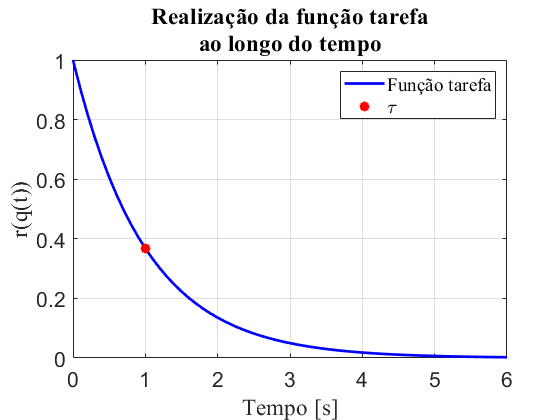
\includegraphics[width=0.7\columnwidth]{Imagens/FuncaoTarefa.png}
% \caption{Gráfico da função tarefa ao longo do tempo.}
% \label{fig:FuncaoTarefa}
% \end{figure}

% A parcela $\dot{q}$ representa a ação de controle $u(q)$, que permite uma convergência exponencial da tarefa. Já $K$, é uma constante que está relacionada a velocidade em que a tarefa é executada, sendo $\tau$ a constante de tempo que compreende a 62,83\% da execução, e $\tau = \frac{1}{K}$ como pode ser observado na Figura~\ref{fig:FuncaoTarefa}. Por fim, a parcela de $\frac{\partial r(q,t)}{\partial t}$ representa um termo de \textit{feedfoward}, que permite que a resposta da saída acompanhe a entrada de referência variante no tempo. Assim, assumindo que $J_r(q)$ é invertível, pode-se obter que a ação de controle conforme descrito na Equação~\ref{eq:3_28}.

% \begin{equation}
% u(q) = J_r(q)^{-1} (-Kr(q(t)) - \frac{\partial r(q,t)}{\partial t})
% \label{eq:3_28}
% \end{equation}

% % \begin{figure}[b!]
% % \centering
% % 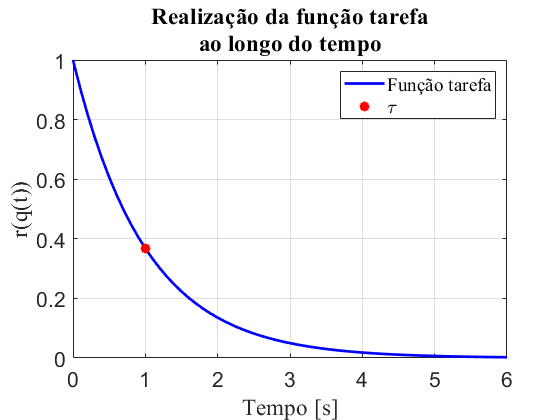
\includegraphics[width=0.7\columnwidth]{Imagens/FuncaoTarefa.png}
% % \caption{Corpo rígido com vetores de velocidade linear e angular.}
% % \label{fig:FuncaoTarefa}
% % \end{figure}

% Apesar disso, nem sempre é possível inverter a Jacobiana de tarefa, uma vez que a Equação~\ref{eq:3_27} pode ser um problema de nenhuma ou infinitas soluções. Nesse caso, o objetivo é obter um valor mais próximo do esperado e que exija um menor esforço computacional. Assim, a fim de obter uma solução de otimização, e omitindo a variável $q$ e $t$ para tornar o processo mais simples de compreensão, é utilizada a pseudoinversa da matriz da Jacobiana de tarefa, definida na Equação~\ref{eq:3_29}\footnote{Uma matriz pseudo inversa é originalmente representada por $J_r^+$, porém, por motivos de desambiguação, foi optado por representar neste projeto por $J_r^{\dagger}$.}, a qual substituindo-a na Equação~\ref{eq:3_28}, obtém-se a relação da Equação~\ref{eq:3_30}.

% \begin{equation}
% J_r^{\dagger} = (J_r^T J_r + \epsilon I_{n\times n})^{-1} J_r^T
% \label{eq:3_29}
% \end{equation}

% \begin{equation}
% u = J_r^{\dagger} (-Kr - \frac{\partial r}{\partial t})
% \label{eq:3_30}
% \end{equation}

% É importante ressaltar que, na Equação~\ref{eq:3_29}, tem-se $\epsilon \rightarrow 0^+$, e que o valor da ação de controle pode se tornar muito instável e ruidoso. Para corrigir isso e evitar um esforço computacional excedente, é utilizado a pseudoinverda amortecida, a qual $\epsilon$ assume um valor baixo, mas que não tende a um valor nulo. Nessa nova expressão, a pseudoinversa amortecida pode ser descrita da seguinte forma:

% \begin{equation}
% J_r^{\dagger (\epsilon)} = \frac{J_r}{J_r^2 + \epsilon}
% \label{eq:3_31}
% \end{equation}

% A qual o maior valor possível é $J_r^{\dagger (\epsilon)} = \frac{1}{2 \sqrt{\epsilon}}$. Assim, quanto maior o valor de $\epsilon$, menor a variação da ação de controle, porém que pode ser mais distante da solução ideal. Assim, a estratégia de controle pode ser definida pela Equação~\ref{eq:3_32}.

% \begin{equation}
% u = J_r^{\dagger (\epsilon)} (-Kr - \frac{\partial r}{\partial t})
% \label{eq:3_32}
% \end{equation}

% Com base nas Jacobianas de posição e orientação fornecidas pelas Equações~\ref{eq:3_23} e~\ref{eq:3_24}, é possível encontrar a Jacobiana de tarefa do efetuador através da Equação~\ref{eq:3_33}.

% \begin{equation}
% J_r(q,t) =
% \begin{bmatrix}
% J_p(q)\\
% x_{des}^T S(x_{ef}(q)) J_{\omega}(q)\\
% y_{des}^T S(y_{ef}(q)) J_{\omega}(q)\\
% z_{des}^T S(z_{ef}(q)) J_{\omega}(q)\\
% \end{bmatrix}
% \label{eq:3_33}
% \end{equation}

% % \begin{figure}[h!]
% % \centering
% % 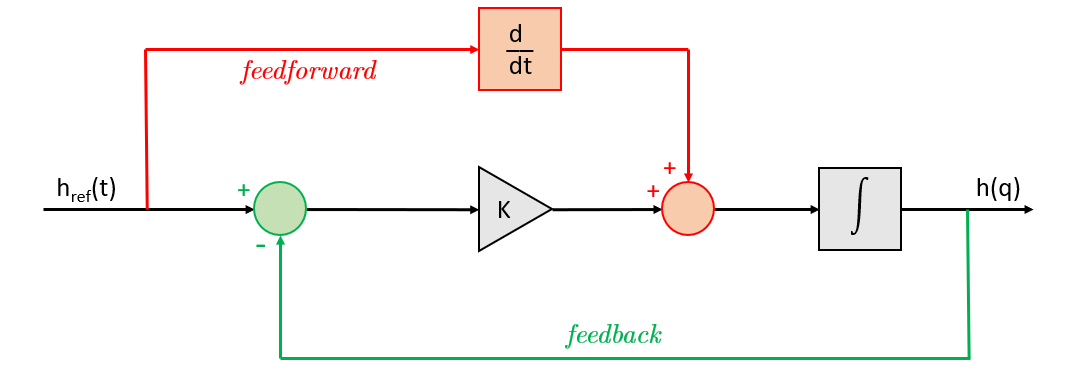
\includegraphics[width=0.7\columnwidth]{Imagens/DiagramaBlocos.PNG}
% % \caption{Diagrama de blocos de controle do manipulador.}
% % \label{fig:DiagramaBlocos}
% % \end{figure}

% Por fim, é possível obter o diagrama de blocos de controle do manipulador, disponível na Figura~\ref{fig:DiagramaBlocos}, a fim de compreender o funcionamento do projeto. A função tarefa desse diagrama é detalhada na Equação~\ref{eq:3_34}.

% \begin{equation}
% r(q,t) = h(q) - h_{ref}(t)
% \label{eq:3_34}
% \end{equation}

% \begin{figure}[h!]
% \centering
% 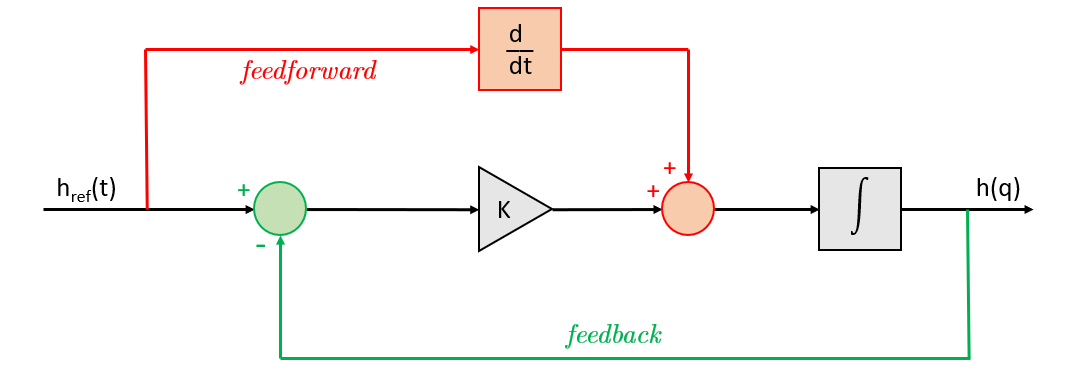
\includegraphics[width=0.7\columnwidth]{Imagens/DiagramaBlocos.PNG}
% \caption{Diagrama de blocos de controle do manipulador.}
% \label{fig:DiagramaBlocos}
% \end{figure}

% %===========================================================
% \section{\textit{Simulação do Sistema e Prototipação}}\label{sec:Cap3_Simulador}

% O manipulador é composto por eixos e juntas, a qual possuem representação espacial como demonstrado na seção~\ref{sec:Cap3_Espacial}. A plataforma CoppeliaSim, antes chamada de V-REP, possui modelos de manipuladores capazes de representar suas limitações e ações possíveis. Ela é amplamente utilizada na área de robótica e possui uma versão educacional que oferece total capacidade de simulação e de edição.

% A plataforma possui suporte a integração com o MATLAB, além de possuir bibliotecas prontas para linguagem Python. O MATLAB, por sua vez, é uma plataforma que consegue lidar bem com processamento de dados que envolvam matrizes, processamento de sinais, análise númerica e construção de gráficos. Ele possui um pacote de suporte ao uso de Arduino, um microcontrolador de baixo custo recomendado na construção de protótipos.

% Como já foi abordado na seção~\ref{sec:Cap3_Deteccao}, existem muitas bibliotecas criadas para a linguagem Python para detecção de objetos. Dessa forma, é possível integrar as bibliotecas utilizadas em um mesmo ambiente, a fim de reduzir o número de plataformas e ambientes de desenvolvimento integrado (IDE) utilizados. Um editor de código-fonte que tem crescido bastante e ganhado suporte da comunidade desenvolvedora através de extensões, é o  Visual Studio Code (VSCode), criado pela Microsoft. Ele é aberto e gratuito, além de possuir suporte para depuração, controle de versão, entre muitos outros recursos. Ele foi escolhido pela facilidade do uso de suas extensões distribuídas pela comunidade, além de exigir menos esforço em sua execução frente a IDEs que recorrem de mesmas funções utilizadas para este projeto.

% Assim, é possível projetar os ambientes para a execução de cada etapa para os objetivos de simular e realizar a validação através de um protótipo. Para a simulação, foi planejado utilizar elementos do CoppeliaSim para simular um enquadramento da imagem de uma câmera. Dessa forma, todo o tratamento deste enquadramento é realizado no VSCode, e os dados do melhor posicionamento são enviados para o MATLAB. Assim, a estrutura de controle é tratada e enviada para realização da simulação do manipulador robótico no CoppeliaSim. Esse processo se repete, de forma a sempre conseguir o posicionamento mais adequado no efetuador do manipulador – onde se encontra a câmera. As etapas podem ser observadas na Figura~\ref{fig:DiagramaSimulacao}.

% % \begin{figure}[h!]
% % \centering
% % 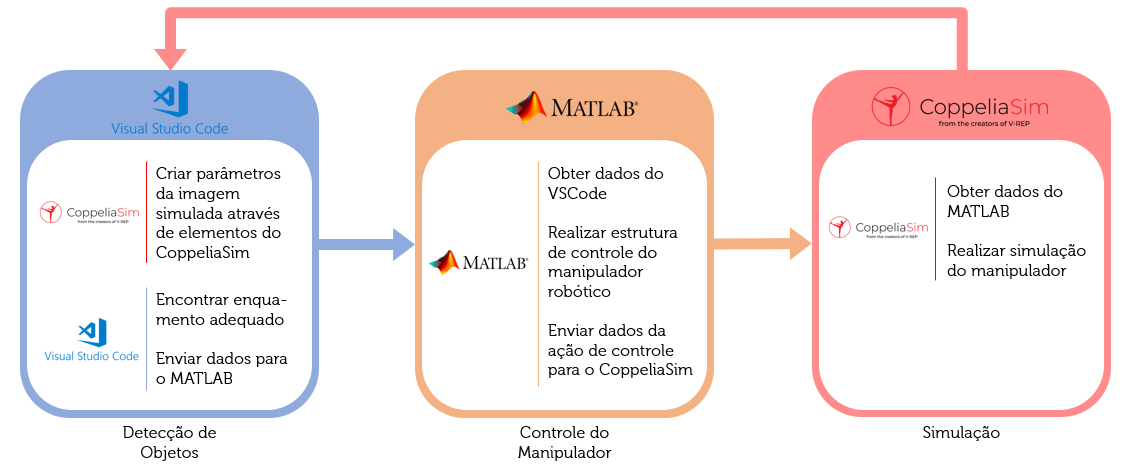
\includegraphics[width=0.9\columnwidth]{Imagens/DiagramaSimulacao.PNG}
% % \caption{Diagrama de etapas para simulação do projeto.}
% % \label{fig:DiagramaSimulacao}
% % \end{figure}

% Para a execução do protótipo, muitas etapas são semelhantes a simulação. Primeiro, as imagens da câmera são obtidas através da biblioteca OpenCV, e é realizada a detecção de pessoas nas imagens e suas posições no enquadramento através do TensorFlow. Logo, é obtido o melhor posicionamento dentro do enquadramento de imagem, e esses dados são enviados para o MATLAB, a qual será responsável por toda parte de controle do manipulador robótico. Este, por sua vez, envia os dados da ação de controle para o Arduino, que é responsável pela ativação dos motores para movimentação do manipulador. Esse processo se repete, de forma a sempre conseguir o posicionamento mais adequado no protótipo – que serve de suporte para a câmera. As etapas podem ser observadas na Figura~\ref{fig:DiagramaPrototipo}.

% \begin{figure}[h!]
% \centering
% 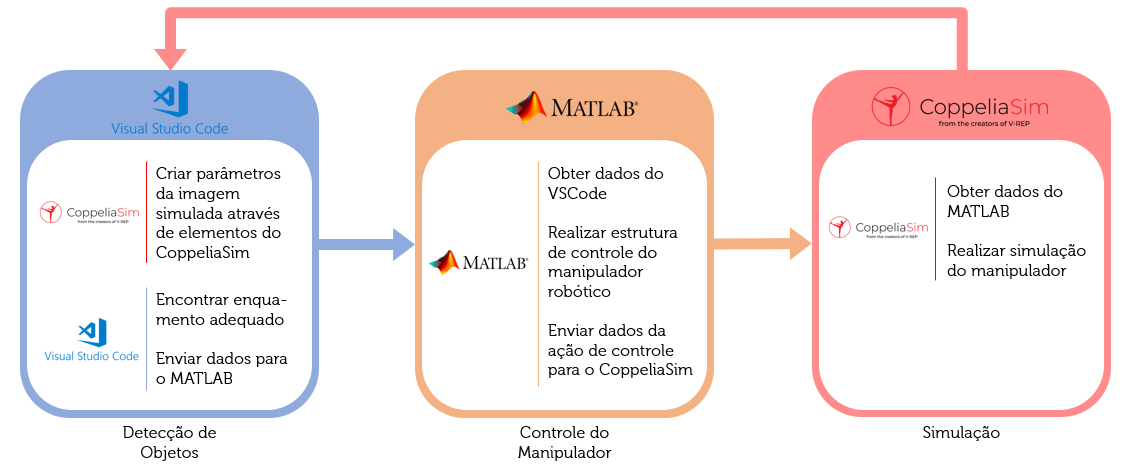
\includegraphics[width=0.9\columnwidth]{Imagens/DiagramaSimulacao.PNG}
% \caption{Diagrama de etapas para simulação do projeto.}
% \label{fig:DiagramaSimulacao}
% \end{figure}

% \begin{figure}[h!]
% \centering
% 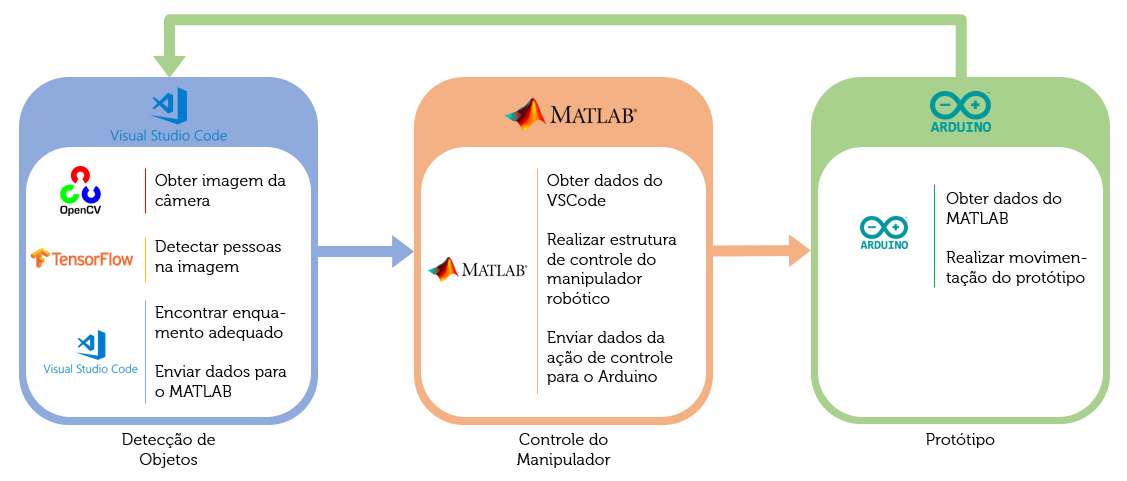
\includegraphics[width=0.9\columnwidth]{Imagens/DiagramaPrototipo.PNG}
% \caption{Diagrama de etapas para execução do protótipo.}
% \label{fig:DiagramaPrototipo}
% \end{figure}



% \textcolor{white}{.}

